\subsubsection{Matriz de Cossenos Diretores}
\label{sec:matriz_cosseno_diretor}

Segundo \cite{wie2008space}, a relação entre dois referenciais em rotação pode ser descrita pela matriz de cossenos diretores (DCM — \emph{Direction Cosine Matrix}), que expressa a orientação de um referencial $B$ em relação a outro $A$.  
Essa matriz ($\mathbf{C}^{B/A}$), é composta pelos cossenos dos ângulos entre os eixos dos dois referenciais e relaciona os vetores unitários conforme

\begin{equation}
\begin{bmatrix}
\vec{x}_B \\ \vec{y}_B \\ \vec{z}_B
\end{bmatrix}
=
\mathbf{C}^{B/A}
\begin{bmatrix}
\vec{x}_A \\ \vec{y}_A \\ \vec{z}_A
\end{bmatrix}
\end{equation}

Cada linha de $\mathbf{C}^{B/A}$ contém as projeções de um eixo do referencial $B$ sobre os eixos de $A$, garantindo que a matriz seja ortonormal.  

\begin{figure}[ht]
    \label{fig:DCM}
\centering
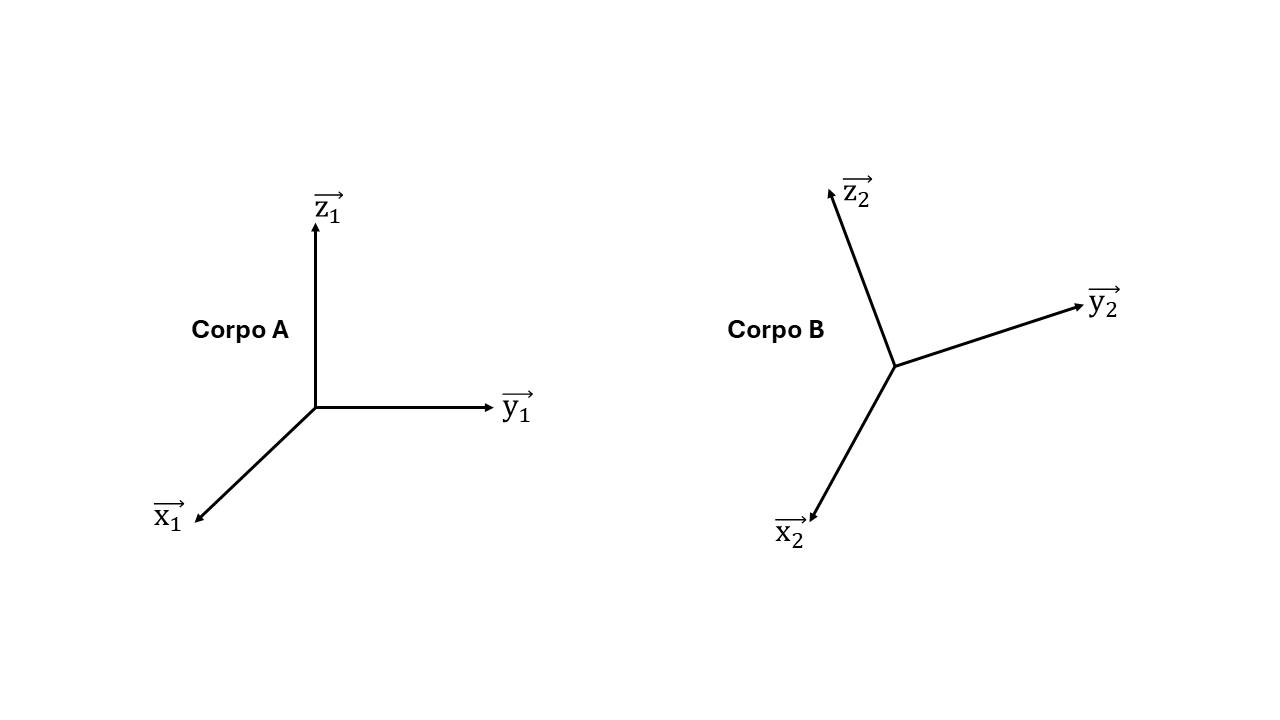
\includegraphics[width=0.90\linewidth]{2 Formulacao matematica/Imagens/DCM.png}
\caption{Dois referenciais movendo um em relação ao outro. Adaptado de \cite{wie2008space}.}
\end{figure}

Como os referenciais giram entre si, os elementos $C_{ij}$ variam no tempo, e a derivada temporal de $\mathbf{C}$ é regida pela equação cinemática diferencial

\begin{equation}
\dot{\mathbf{C}} + \boldsymbol{\Omega}\mathbf{C} = 0
\label{eq:cinematica_dcm}
\end{equation}

A matriz $\boldsymbol{\Omega}$ é antissimétrica e representa o operador de produto vetorial associado à velocidade angular $\vec{\omega}$ expressa no referencial do corpo

\begin{equation}
\boldsymbol{\Omega} =
\begin{bmatrix}
0 & -\omega_z & \omega_y \\
\omega_z & 0 & -\omega_x \\
-\omega_y & \omega_x & 0
\end{bmatrix}
\end{equation}

A integração da equação \eqref{eq:cinematica_dcm} fornece a evolução temporal da orientação do corpo.  
A condição de ortonormalidade

\begin{equation}
\mathbf{C}\mathbf{C}^T = \mathbf{I}
\end{equation}

é invariável no tempo e é usada como verificação de consistência numérica nas simulações de atitude.